\begin{figure}[!htbp]
	\centering
	\usetikzlibrary{arrows.meta,calc,decorations.markings}
	
	% --- helper per le figure ---
	\tikzset{midarrow/.style={postaction={decorate},
			decoration={markings, mark=at position 0.56 with {\arrow{Stealth}}}}}
	
	\newcommand{\rightangle}[3]{%
		\coordinate (ra1) at ($(#2)!2mm!(#1)$);
		\coordinate (ra3) at ($(#2)!2mm!(#3)$);
		\draw[line width=0.4pt] (ra1) -- ($(ra1)+(ra3)-(#2)$) -- (ra3);}
	\resizebox{0.9\textwidth}{!}{%
		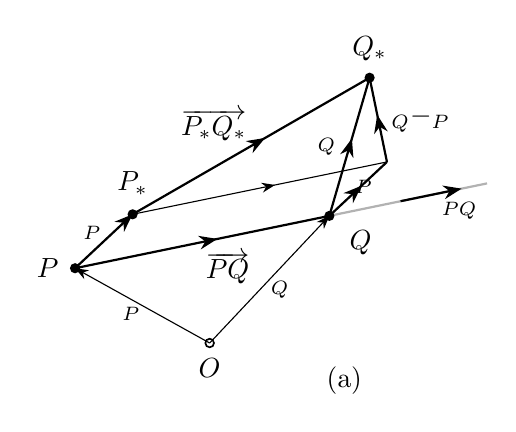
\begin{tikzpicture}[>=Stealth, line width=0.8pt, scale=0.95,
			pt/.style={circle,fill,inner sep=1.3pt},
			open/.style={circle,draw,line width=0.6pt,inner sep=1.1pt}]
			\coordinate (O)  at (1.8,-0.5);
			\coordinate (P)  at (0,0.5);
			\coordinate (Q)  at (3.4,1.2);
			\coordinate (aA) at (3.645,1.250);
			\coordinate (aB) at (4.477,1.422);
			\coordinate (Ps) at (0.770,1.221);
			\coordinate (Qs) at (3.938,3.047);
			\coordinate (QuP) at (4.170,1.921);
			
			\draw[->, thin] (O) -- (P) node[pos=0.5,below left=-3pt] {$\xb_P$};
			\draw[->, thin] (O) -- (Q) node[pos=0.5,below right=-3pt] {$\xb_Q$};
			
			\draw[thick, midarrow] (P) -- (Q) node[pos=0.6,below=2pt] {$\overrightarrow{PQ}$};
			%\draw[->, thick] (aA) -- (aB) node[pos=0.97,above=1pt] {$\ab_{PQ}$};
			
			% retta d'azione di PQ (grigia) da Q verso destra
			\draw[gray!60] (Q) -- ($(P)!1.62!(Q)$);
			
			% versore a_PQ (nero) disegnato su quella retta
			\coordinate (aA) at ($(P)!1.28!(Q)$);
			\coordinate (aB) at ($(P)!1.52!(Q)$);
			\draw[->, thick] (aA) -- (aB) node[pos=0.97,below=1pt] {$\ab_{PQ}$};
			
			\draw[thin, midarrow] (Ps) -- (QuP);   % chiude il parallelogramma P Q (Q+u_P) P*
			
			\draw[->, thick] (P) -- (Ps) node[pos=0.5,above left=-3pt] {$\ub_P$};
			\draw[thick, midarrow] (Q) -- (Qs) node[pos=0.5,left=1pt] {$\ub_Q$};
			\draw[thick, midarrow] (Q) -- (QuP) node[pos=0.55,below right=-6pt] {$\ub_P$};
			\draw[thick, midarrow] (QuP) -- (Qs) node[pos=0.5,right=1pt] {$\ub_Q-\ub_P$};
			
			\draw[thick, midarrow] (Ps) -- (Qs) node[pos=0.5,above left=-2pt] {$\overrightarrow{P_*Q_*}$};
			
			\node[open,label={below:$O$}] at (O) {};
			\node[pt,label={left:$P$}]  at (P) {};
			\node[pt,label={[xshift=2pt]below right:$Q$}] at (Q) {};
			\node[pt,label={[yshift=1pt]above :$P_*$}]  at (Ps) {};
			\node[pt,label={ above:$Q_*$}] at (Qs) {};
			
			\node at (3.6,-1.0) {(a)};
		\end{tikzpicture}
		\quad
		% ---- pannello (b) ----
		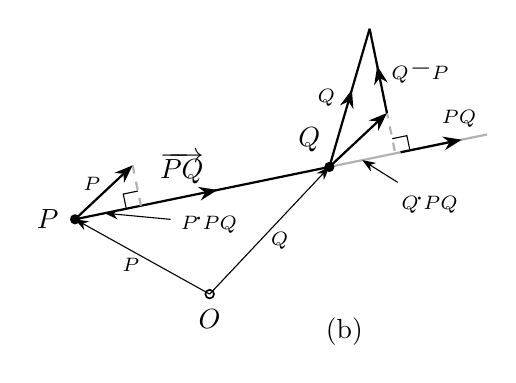
\begin{tikzpicture}[>=Stealth, line width=0.8pt, scale=0.95,
			pt/.style={circle,fill,inner sep=1.3pt},
			open/.style={circle,draw,line width=0.6pt,inner sep=1.1pt}]
			\coordinate (O)  at (1.8,-0.5);
			\coordinate (P)  at (0,0.5);
			\coordinate (Q)  at (3.4,1.2);
			\coordinate (aA) at (3.645,1.250);
			\coordinate (aB) at (4.477,1.422);
			\coordinate (Ps) at (0.770,1.221);
			\coordinate (Qs) at (3.938,3.047);
			\coordinate (QuP) at (4.170,1.921);
			\coordinate (FP) at (0.881,0.682);
			\coordinate (FQ) at (4.281,1.382);
			
			\draw[->, thin] (O) -- (P) node[pos=0.5,below left=-3pt] {$\xb_P$};
			\draw[->, thin] (O) -- (Q) node[pos=0.5,below right=-3pt] {$\xb_Q$};
			
			\draw[thick, midarrow] (P) -- (Q) node[pos=0.42,above=1pt] {$\overrightarrow{PQ}$};
			%\draw[->, thick] (aA) -- (aB) node[pos=0.97,above=1pt] {$\ab_{PQ}$};
			% retta d'azione di PQ (grigia) da Q verso destra
			\draw[gray!60] (Q) -- ($(P)!1.62!(Q)$);
			
			% versore a_PQ (nero) disegnato su quella retta
			\coordinate (aA) at ($(P)!1.28!(Q)$);
			\coordinate (aB) at ($(P)!1.52!(Q)$);
			\draw[->, thick] (aA) -- (aB) node[pos=0.97,above=1pt] {$\ab_{PQ}$};
			
			% proiezioni grigie tratteggiate (PRIMA di u_Q-u_P) + angoli retti
			\draw[dashed, gray!60] (Ps) -- (FP);
			\draw[dashed, gray!60] (Qs) -- (FQ);
			\rightangle{P}{FP}{Ps}
			\rightangle{aB}{FQ}{Qs}
			
			% spostamenti (DOPO: sovrascrivono il grigio)
			\draw[->, thick] (P) -- (Ps) node[pos=0.5,above left=-3pt] {$\ub_P$};
			\draw[thick, midarrow] (Q) -- (Qs) node[pos=0.5,left=1pt] {$\ub_Q$};
			\draw[->, thick] (Q) -- (QuP);
			\draw[thick, midarrow] (QuP) -- (Qs) node[pos=0.5,right=1pt] {$\ub_Q-\ub_P$};
			
			% etichette delle proiezioni collegate con una freccia di richiamo
			%\node (lpP) at (1.85,0.02) {$\ub_P\!\cdot\ab_{PQ}$};
			%\draw[gray!60] (P) -- (FP);
			\node (lpP) at (1.80,0.45) {$\ub_P\!\cdot\ab_{PQ}$};
			\draw[->, thin] (lpP) -- ($(P)!0.45!(FP)$);
			\node (lpQ) at (4.75,0.72) {$\ub_Q\!\cdot\ab_{PQ}$};
			\draw[->, thin] (lpQ) -- ($(Q)!0.5!(FQ)$);
			
			\node[open,label={below:$O$}] at (O) {};
			\node[pt,label={left:$P$}]  at (P) {};
			\node[pt,label={[xshift=2pt]above left:$Q$}] at (Q) {};
			\node at (3.6,-1.0) {(b)};
		\end{tikzpicture}
	}
	\caption{(a)~Spostamenti rigidi e (b)~interpretazione geometrica della condizione di ortogonalità fra il vettore posizione relativo $\protect\overrightarrow{PQ}$ e il vettore relativo degli spostamenti infinitesimi $\ub_Q - \ub_P$.}
	\label{fig:orto_PQ_spost_relat}
\end{figure}
